\PassOptionsToPackage{unicode=true}{hyperref} % options for packages loaded elsewhere
\PassOptionsToPackage{hyphens}{url}
%
\documentclass[]{article}
\usepackage{lmodern}
\usepackage{amssymb,amsmath}
\usepackage{ifxetex,ifluatex}
\usepackage{fixltx2e} % provides \textsubscript
\ifnum 0\ifxetex 1\fi\ifluatex 1\fi=0 % if pdftex
  \usepackage[T1]{fontenc}
  \usepackage[utf8]{inputenc}
  \usepackage{textcomp} % provides euro and other symbols
\else % if luatex or xelatex
  \usepackage{unicode-math}
  \defaultfontfeatures{Ligatures=TeX,Scale=MatchLowercase}
\fi
% use upquote if available, for straight quotes in verbatim environments
\IfFileExists{upquote.sty}{\usepackage{upquote}}{}
% use microtype if available
\IfFileExists{microtype.sty}{%
\usepackage[]{microtype}
\UseMicrotypeSet[protrusion]{basicmath} % disable protrusion for tt fonts
}{}
\IfFileExists{parskip.sty}{%
\usepackage{parskip}
}{% else
\setlength{\parindent}{0pt}
\setlength{\parskip}{6pt plus 2pt minus 1pt}
}
\usepackage{hyperref}
\hypersetup{
            pdftitle={forchapter5},
            pdfauthor={Haziq Jamil},
            pdfborder={0 0 0},
            breaklinks=true}
\urlstyle{same}  % don't use monospace font for urls
\usepackage[margin=1in]{geometry}
\usepackage{color}
\usepackage{fancyvrb}
\newcommand{\VerbBar}{|}
\newcommand{\VERB}{\Verb[commandchars=\\\{\}]}
\DefineVerbatimEnvironment{Highlighting}{Verbatim}{commandchars=\\\{\}}
% Add ',fontsize=\small' for more characters per line
\usepackage{framed}
\definecolor{shadecolor}{RGB}{248,248,248}
\newenvironment{Shaded}{\begin{snugshade}}{\end{snugshade}}
\newcommand{\AlertTok}[1]{\textcolor[rgb]{0.94,0.16,0.16}{#1}}
\newcommand{\AnnotationTok}[1]{\textcolor[rgb]{0.56,0.35,0.01}{\textbf{\textit{#1}}}}
\newcommand{\AttributeTok}[1]{\textcolor[rgb]{0.77,0.63,0.00}{#1}}
\newcommand{\BaseNTok}[1]{\textcolor[rgb]{0.00,0.00,0.81}{#1}}
\newcommand{\BuiltInTok}[1]{#1}
\newcommand{\CharTok}[1]{\textcolor[rgb]{0.31,0.60,0.02}{#1}}
\newcommand{\CommentTok}[1]{\textcolor[rgb]{0.56,0.35,0.01}{\textit{#1}}}
\newcommand{\CommentVarTok}[1]{\textcolor[rgb]{0.56,0.35,0.01}{\textbf{\textit{#1}}}}
\newcommand{\ConstantTok}[1]{\textcolor[rgb]{0.00,0.00,0.00}{#1}}
\newcommand{\ControlFlowTok}[1]{\textcolor[rgb]{0.13,0.29,0.53}{\textbf{#1}}}
\newcommand{\DataTypeTok}[1]{\textcolor[rgb]{0.13,0.29,0.53}{#1}}
\newcommand{\DecValTok}[1]{\textcolor[rgb]{0.00,0.00,0.81}{#1}}
\newcommand{\DocumentationTok}[1]{\textcolor[rgb]{0.56,0.35,0.01}{\textbf{\textit{#1}}}}
\newcommand{\ErrorTok}[1]{\textcolor[rgb]{0.64,0.00,0.00}{\textbf{#1}}}
\newcommand{\ExtensionTok}[1]{#1}
\newcommand{\FloatTok}[1]{\textcolor[rgb]{0.00,0.00,0.81}{#1}}
\newcommand{\FunctionTok}[1]{\textcolor[rgb]{0.00,0.00,0.00}{#1}}
\newcommand{\ImportTok}[1]{#1}
\newcommand{\InformationTok}[1]{\textcolor[rgb]{0.56,0.35,0.01}{\textbf{\textit{#1}}}}
\newcommand{\KeywordTok}[1]{\textcolor[rgb]{0.13,0.29,0.53}{\textbf{#1}}}
\newcommand{\NormalTok}[1]{#1}
\newcommand{\OperatorTok}[1]{\textcolor[rgb]{0.81,0.36,0.00}{\textbf{#1}}}
\newcommand{\OtherTok}[1]{\textcolor[rgb]{0.56,0.35,0.01}{#1}}
\newcommand{\PreprocessorTok}[1]{\textcolor[rgb]{0.56,0.35,0.01}{\textit{#1}}}
\newcommand{\RegionMarkerTok}[1]{#1}
\newcommand{\SpecialCharTok}[1]{\textcolor[rgb]{0.00,0.00,0.00}{#1}}
\newcommand{\SpecialStringTok}[1]{\textcolor[rgb]{0.31,0.60,0.02}{#1}}
\newcommand{\StringTok}[1]{\textcolor[rgb]{0.31,0.60,0.02}{#1}}
\newcommand{\VariableTok}[1]{\textcolor[rgb]{0.00,0.00,0.00}{#1}}
\newcommand{\VerbatimStringTok}[1]{\textcolor[rgb]{0.31,0.60,0.02}{#1}}
\newcommand{\WarningTok}[1]{\textcolor[rgb]{0.56,0.35,0.01}{\textbf{\textit{#1}}}}
\usepackage{graphicx,grffile}
\makeatletter
\def\maxwidth{\ifdim\Gin@nat@width>\linewidth\linewidth\else\Gin@nat@width\fi}
\def\maxheight{\ifdim\Gin@nat@height>\textheight\textheight\else\Gin@nat@height\fi}
\makeatother
% Scale images if necessary, so that they will not overflow the page
% margins by default, and it is still possible to overwrite the defaults
% using explicit options in \includegraphics[width, height, ...]{}
\setkeys{Gin}{width=\maxwidth,height=\maxheight,keepaspectratio}
\setlength{\emergencystretch}{3em}  % prevent overfull lines
\providecommand{\tightlist}{%
  \setlength{\itemsep}{0pt}\setlength{\parskip}{0pt}}
\setcounter{secnumdepth}{0}
% Redefines (sub)paragraphs to behave more like sections
\ifx\paragraph\undefined\else
\let\oldparagraph\paragraph
\renewcommand{\paragraph}[1]{\oldparagraph{#1}\mbox{}}
\fi
\ifx\subparagraph\undefined\else
\let\oldsubparagraph\subparagraph
\renewcommand{\subparagraph}[1]{\oldsubparagraph{#1}\mbox{}}
\fi

% set default figure placement to htbp
\makeatletter
\def\fps@figure{htbp}
\makeatother


\title{forchapter5}
\author{Haziq Jamil}
\date{18/03/2020}

\begin{document}
\maketitle

\begin{verbatim}
## Parsed with column specification:
## cols(
##   state = col_character(),
##   poverty = col_double(),
##   hs_grad = col_double(),
##   home_own = col_double(),
##   median_income = col_double(),
##   party_maj = col_character()
## )
\end{verbatim}

\begin{Shaded}
\begin{Highlighting}[]
\NormalTok{poverty}
\end{Highlighting}
\end{Shaded}

\begin{verbatim}
## # A tibble: 51 x 6
##    state                poverty hs_grad home_own median_income party_maj
##    <chr>                  <dbl>   <dbl>    <dbl>         <dbl> <chr>    
##  1 Alabama                19.9     76.8     73.4        36963. Rep      
##  2 Alaska                 12.3     86.6     63.2        59351. Rep      
##  3 Arizona                19.0     81.8     69.7        42418. Rep      
##  4 Arkansas               20.0     78.9     71.2        34983. Rep      
##  5 California             14.2     82.5     63.3        55266. Dem      
##  6 Colorado               12.9     88.1     72.1        50136. Dem      
##  7 Connecticut             8.31    89.1     71.7        68935. Dem      
##  8 Delaware               11.5     86.2     74.7        55568. Dem      
##  9 District of Columbia   18.5     86.5     43.5        58526  Dem      
## 10 Florida                16.0     82.2     74.6        44269. Rep      
## # ... with 41 more rows
\end{verbatim}

\begin{Shaded}
\begin{Highlighting}[]
\NormalTok{GGally}\OperatorTok{::}\KeywordTok{ggpairs}\NormalTok{(poverty[, }\DecValTok{-1}\NormalTok{]) }\OperatorTok{+}\StringTok{ }\KeywordTok{theme_bw}\NormalTok{()}
\end{Highlighting}
\end{Shaded}

\begin{verbatim}
## Registered S3 method overwritten by 'GGally':
##   method from   
##   +.gg   ggplot2
\end{verbatim}

\begin{verbatim}
## `stat_bin()` using `bins = 30`. Pick better value with `binwidth`.
## `stat_bin()` using `bins = 30`. Pick better value with `binwidth`.
## `stat_bin()` using `bins = 30`. Pick better value with `binwidth`.
## `stat_bin()` using `bins = 30`. Pick better value with `binwidth`.
\end{verbatim}

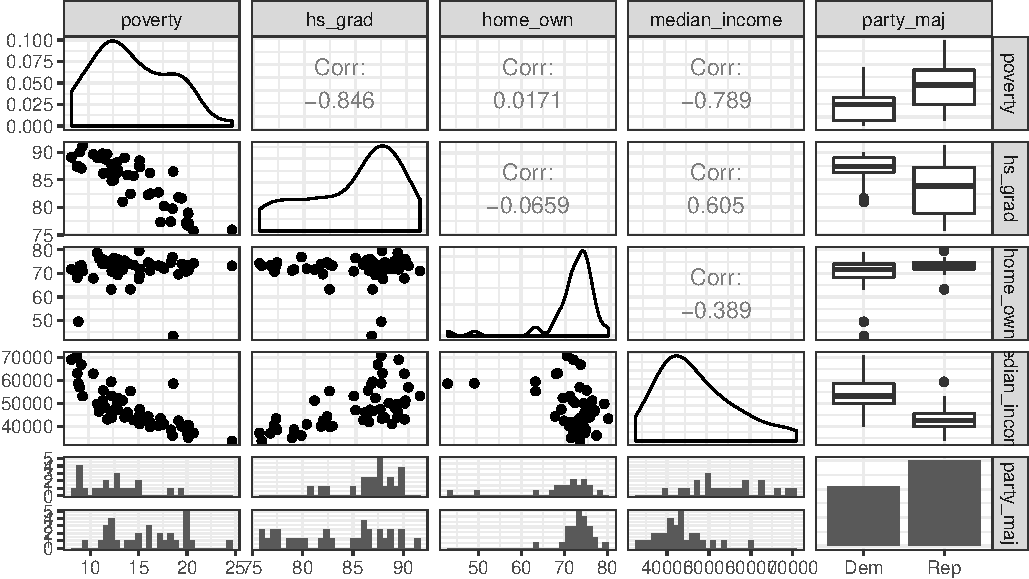
\includegraphics{forchapter5_files/figure-latex/05-pairplot-1.pdf}

\begin{Shaded}
\begin{Highlighting}[]
\NormalTok{mod <-}\StringTok{ }\KeywordTok{lm}\NormalTok{(}\DataTypeTok{formula =}\NormalTok{ poverty }\OperatorTok{~}\StringTok{ }\NormalTok{hs_grad }\OperatorTok{+}\StringTok{ }\NormalTok{home_own }\OperatorTok{+}\StringTok{ }\KeywordTok{I}\NormalTok{(median_income}\OperatorTok{/}\DecValTok{1000}\NormalTok{) }\OperatorTok{+}
\StringTok{            }\NormalTok{party_maj, }\DataTypeTok{data =}\NormalTok{ poverty)}
\KeywordTok{summary}\NormalTok{(mod)}
\end{Highlighting}
\end{Shaded}

\begin{verbatim}
## 
## Call:
## lm(formula = poverty ~ hs_grad + home_own + I(median_income/1000) + 
##     party_maj, data = poverty)
## 
## Residuals:
##     Min      1Q  Median      3Q     Max 
## -4.8794 -0.8104 -0.0762  0.8412  3.2827 
## 
## Coefficients:
##                       Estimate Std. Error t value Pr(>|t|)    
## (Intercept)           76.07336    4.58210  16.602  < 2e-16 ***
## hs_grad               -0.45345    0.05599  -8.098 2.12e-10 ***
## home_own              -0.14614    0.03538  -4.130 0.000151 ***
## I(median_income/1000) -0.26101    0.03427  -7.616 1.10e-09 ***
## party_majRep          -0.51100    0.51347  -0.995 0.324857    
## ---
## Signif. codes:  0 '***' 0.001 '**' 0.01 '*' 0.05 '.' 0.1 ' ' 1
## 
## Residual standard error: 1.354 on 46 degrees of freedom
## Multiple R-squared:  0.8859, Adjusted R-squared:  0.876 
## F-statistic: 89.28 on 4 and 46 DF,  p-value: < 2.2e-16
\end{verbatim}

\begin{Shaded}
\begin{Highlighting}[]
\NormalTok{X <-}\StringTok{ }\KeywordTok{model.matrix}\NormalTok{(mod); }\KeywordTok{head}\NormalTok{(X)  }\CommentTok{# n by (p + 1) matrix}
\end{Highlighting}
\end{Shaded}

\begin{verbatim}
##   (Intercept)  hs_grad home_own I(median_income/1000) party_majRep
## 1           1 76.78209 73.38657              36.96294            1
## 2           1 86.59310 63.22759              59.35103            1
## 3           1 81.82000 69.65333              42.41793            1
## 4           1 78.86400 71.23067              34.98271            1
## 5           1 82.45862 63.26724              55.26572            0
## 6           1 88.13906 72.14531              50.13584            0
\end{verbatim}

\begin{Shaded}
\begin{Highlighting}[]
\NormalTok{y <-}\StringTok{ }\NormalTok{poverty}\OperatorTok{$}\NormalTok{poverty; }\KeywordTok{head}\NormalTok{(y)  }\CommentTok{# n by 1 vector}
\end{Highlighting}
\end{Shaded}

\begin{verbatim}
## [1] 19.90746 12.29310 19.03333 20.00533 14.22069 12.86094
\end{verbatim}

\begin{Shaded}
\begin{Highlighting}[]
\NormalTok{XtX <-}\StringTok{ }\KeywordTok{t}\NormalTok{(X) }\OperatorTok\StringTok{ }\NormalTok{X  }\CommentTok{# (p + 1) by (p + 1) matrix}
\KeywordTok{colnames}\NormalTok{(XtX) <-}\StringTok{ }\KeywordTok{rownames}\NormalTok{(XtX) <-}\StringTok{ }\OtherTok{NULL}
\NormalTok{XtX}
\end{Highlighting}
\end{Shaded}

\begin{verbatim}
##          [,1]       [,2]       [,3]       [,4]     [,5]
## [1,]   51.000   4323.498   3657.123   2430.910   30.000
## [2,] 4323.498 367497.623 309942.167 207273.903 2498.765
## [3,] 3657.123 309942.167 264098.108 173256.517 2202.333
## [4,] 2430.910 207273.903 173256.517 119871.817 1284.466
## [5,]   30.000   2498.765   2202.333   1284.466   30.000
\end{verbatim}

\begin{Shaded}
\begin{Highlighting}[]
\NormalTok{Xty <-}\StringTok{ }\KeywordTok{t}\NormalTok{(X) }\OperatorTok\StringTok{ }\NormalTok{y; }\KeywordTok{head}\NormalTok{(Xty)  }\CommentTok{# (p + 1) by 1 vector}
\end{Highlighting}
\end{Shaded}

\begin{verbatim}
##                             [,1]
## (Intercept)             734.9980
## hs_grad               61590.5786
## home_own              52725.4769
## I(median_income/1000) 33676.2834
## party_majRep            476.7111
\end{verbatim}

\begin{Shaded}
\begin{Highlighting}[]
\KeywordTok{as.numeric}\NormalTok{(beta.hat <-}\StringTok{ }\KeywordTok{solve}\NormalTok{(XtX, Xty))  }\CommentTok{# regression coefficients}
\end{Highlighting}
\end{Shaded}

\begin{verbatim}
## [1] 76.0733587 -0.4534462 -0.1461374 -0.2610123 -0.5109967
\end{verbatim}

\begin{Shaded}
\begin{Highlighting}[]
\NormalTok{y.hat <-}\StringTok{ }\KeywordTok{as.numeric}\NormalTok{(X }\OperatorTok\StringTok{ }\NormalTok{beta.hat); }\KeywordTok{head}\NormalTok{(y.hat)  }\CommentTok{# fitted values}
\end{Highlighting}
\end{Shaded}

\begin{verbatim}
## [1] 20.37351 11.56579 17.21084 20.26140 15.01207 12.47784
\end{verbatim}

\begin{Shaded}
\begin{Highlighting}[]
\NormalTok{eps.hat <-}\StringTok{ }\NormalTok{y }\OperatorTok{-}\StringTok{ }\NormalTok{y.hat; }\KeywordTok{head}\NormalTok{(eps.hat)  }\CommentTok{# residuals}
\end{Highlighting}
\end{Shaded}

\begin{verbatim}
## [1] -0.4660507  0.7273168  1.8224961 -0.2560688 -0.7913801  0.3830990
\end{verbatim}

\begin{Shaded}
\begin{Highlighting}[]
\NormalTok{(sigma.hat <-}\StringTok{ }\KeywordTok{sqrt}\NormalTok{(}\KeywordTok{sum}\NormalTok{(eps.hat }\OperatorTok{^}\StringTok{ }\DecValTok{2}\NormalTok{) }\OperatorTok{/}\StringTok{ }\NormalTok{(}\DecValTok{51} \OperatorTok{-}\StringTok{ }\DecValTok{4} \OperatorTok{-}\StringTok{ }\DecValTok{1}\NormalTok{)))  }\CommentTok{# residual SE}
\end{Highlighting}
\end{Shaded}

\begin{verbatim}
## [1] 1.353753
\end{verbatim}

\begin{Shaded}
\begin{Highlighting}[]
\KeywordTok{fitted}\NormalTok{(mod)  }\CommentTok{# obtain fitted values}
\end{Highlighting}
\end{Shaded}

\begin{verbatim}
##         1         2         3         4         5         6         7         8 
## 20.373513 11.565787 17.210837 20.261402 15.012070 12.477839  7.194859 11.576235 
##         9        10        11        12        13        14        15        16 
## 15.217284 15.819316 19.729882 13.879387 14.791221 13.493640 13.587406 11.915343 
##        17        18        19        20        21        22        23        24 
## 13.474400 20.683055 19.524389 13.240073  8.420077  9.104415 12.953813 11.231420 
##        25        26        27        28        29        30        31        32 
## 21.637436 17.040754 14.251766 12.859763 13.400985  9.679679  7.710733 17.805235 
##        33        34        35        36        37        38        39        40 
## 12.902249 17.969372 14.065428 13.752141 16.863705 14.909914 13.171882  9.942183 
##        41        42        43        44        45        46        47        48 
## 19.186426 15.105553 19.505661 18.487914 10.424302 11.556045 15.513875 14.018749 
##        49        50        51 
## 18.759122 11.743215  9.996266
\end{verbatim}

\begin{Shaded}
\begin{Highlighting}[]
\KeywordTok{resid}\NormalTok{(mod)  }\CommentTok{# obtain residuals}
\end{Highlighting}
\end{Shaded}

\begin{verbatim}
##           1           2           3           4           5           6 
## -0.46605065  0.72731679  1.82249609 -0.25606877 -0.79138008  0.38309895 
##           7           8           9          10          11          12 
##  1.11764146 -0.07623466  3.28271639  0.17919156  0.05250815 -4.87938690 
##          13          14          15          16          17          18 
## -0.26394784 -0.55344392 -0.99936285 -0.85271642 -1.16773370 -0.14222118 
##          19          20          21          22          23          24 
##  0.53654811  0.39742676  0.88408973  1.40272776  2.14377701 -0.33141953 
##          25          26          27          28          29          30 
##  2.75158873 -0.82944933  0.89109102 -0.96191335 -1.05392611 -0.53967877 
##          31          32          33          34          35          36 
##  1.15117164  1.54627966  0.03323485 -0.38737151 -1.72769199  0.18081322 
##          37          38          39          40          41          42 
##  0.17136036  0.16508568 -0.87188216 -1.04218336  0.79835675  1.08687105 
##          43          44          45          46          47          48 
## -1.23408238 -1.25563045  1.01362932 -0.14890176 -2.07432310  1.12740532 
##          49          50          51 
## -0.32639451 -0.05154804 -0.56148303
\end{verbatim}

\begin{Shaded}
\begin{Highlighting}[]
\NormalTok{diag.plots <-}\StringTok{ }\NormalTok{lindia}\OperatorTok{::}\KeywordTok{gg_diagnose}\NormalTok{(mod, }\DataTypeTok{theme =} \KeywordTok{theme_bw}\NormalTok{(), }\DataTypeTok{plot.all =} \OtherTok{FALSE}\NormalTok{,}
                                  \DataTypeTok{scale.factor =} \DecValTok{1}\NormalTok{)}
\NormalTok{diag.plots}\OperatorTok{$}\NormalTok{res_fitted}
\end{Highlighting}
\end{Shaded}

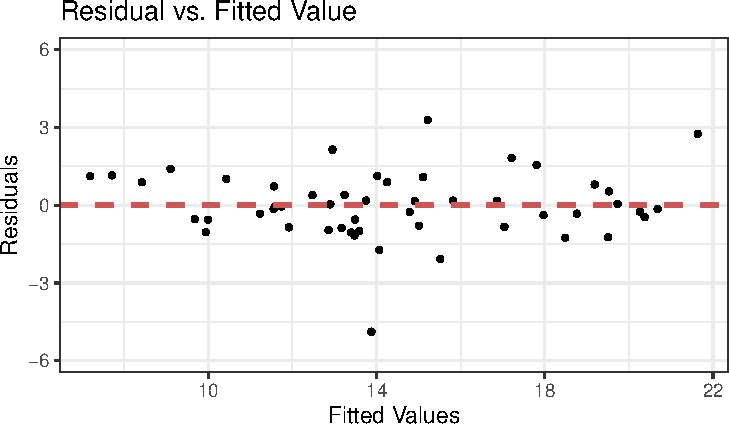
\includegraphics{forchapter5_files/figure-latex/05-diagplot-1.pdf}

\begin{Shaded}
\begin{Highlighting}[]
\NormalTok{diag.plots}\OperatorTok{$}\NormalTok{residual_hist}
\end{Highlighting}
\end{Shaded}

\begin{verbatim}
## `stat_bin()` using `bins = 30`. Pick better value with `binwidth`.
\end{verbatim}

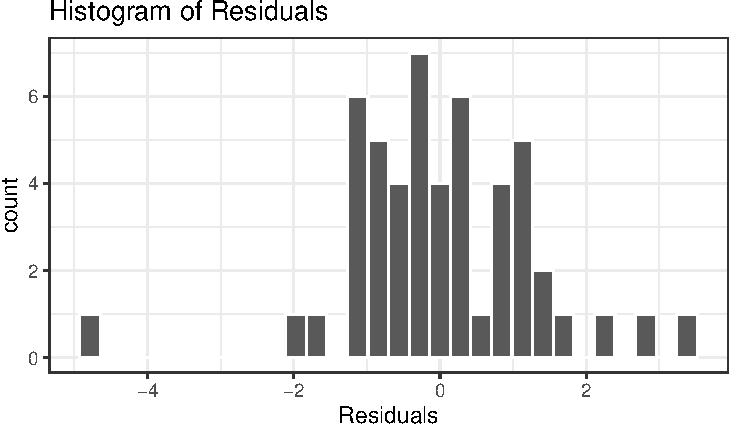
\includegraphics{forchapter5_files/figure-latex/05-diagplot-2.pdf}

\begin{Shaded}
\begin{Highlighting}[]
\NormalTok{diag.plots}\OperatorTok{$}\NormalTok{qqplot}
\end{Highlighting}
\end{Shaded}

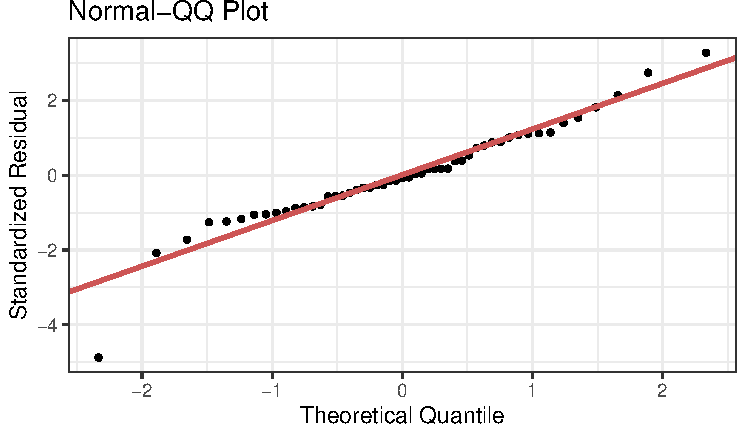
\includegraphics{forchapter5_files/figure-latex/05-diagplot-3.pdf}

\begin{Shaded}
\begin{Highlighting}[]
\NormalTok{(var.beta.hat <-}\StringTok{ }\NormalTok{sigma.hat }\OperatorTok{^}\StringTok{ }\DecValTok{2} \OperatorTok{*}\StringTok{ }\KeywordTok{solve}\NormalTok{(XtX))  }\CommentTok{# Estimate of Var(beta.hat)}
\end{Highlighting}
\end{Shaded}

\begin{verbatim}
##              [,1]          [,2]          [,3]          [,4]         [,5]
## [1,] 20.995620883 -0.1849707465 -0.0674556619 -0.0029825145 -0.509316515
## [2,] -0.184970747  0.0031353530 -0.0004649709 -0.0010121404  0.001289793
## [3,] -0.067455662 -0.0004649709  0.0012520320  0.0003869122 -0.002294815
## [4,] -0.002982514 -0.0010121404  0.0003869122  0.0011746260  0.008589991
## [5,] -0.509316515  0.0012897933 -0.0022948145  0.0085899906  0.263655017
\end{verbatim}

\begin{Shaded}
\begin{Highlighting}[]
\NormalTok{(se.beta.hat <-}\StringTok{ }\KeywordTok{sqrt}\NormalTok{(}\KeywordTok{diag}\NormalTok{(var.beta.hat)))  }\CommentTok{# SE beta.hat}
\end{Highlighting}
\end{Shaded}

\begin{verbatim}
## [1] 4.58209787 0.05599422 0.03538406 0.03427282 0.51347348
\end{verbatim}

\begin{Shaded}
\begin{Highlighting}[]
\KeywordTok{as.numeric}\NormalTok{(beta.hat }\OperatorTok{/}\StringTok{ }\NormalTok{se.beta.hat)  }\CommentTok{# test statistic value}
\end{Highlighting}
\end{Shaded}

\begin{verbatim}
## [1] 16.6022990 -8.0980881 -4.1300351 -7.6157228 -0.9951764
\end{verbatim}

\begin{Shaded}
\begin{Highlighting}[]
\KeywordTok{as.numeric}\NormalTok{(  }\CommentTok{# p-values}
  \KeywordTok{pt}\NormalTok{(}\KeywordTok{abs}\NormalTok{(beta.hat }\OperatorTok{/}\StringTok{ }\NormalTok{se.beta.hat), }\DataTypeTok{df =} \DecValTok{50}\NormalTok{, }\DataTypeTok{lower.tail =} \OtherTok{FALSE}\NormalTok{)}
\NormalTok{)}
\end{Highlighting}
\end{Shaded}

\begin{verbatim}
## [1] 2.753456e-22 5.867138e-11 6.883705e-05 3.281345e-10 1.622212e-01
\end{verbatim}

\begin{Shaded}
\begin{Highlighting}[]
\NormalTok{(total.SS <-}\StringTok{ }\KeywordTok{sum}\NormalTok{((y }\OperatorTok{-}\StringTok{ }\KeywordTok{mean}\NormalTok{(y)) }\OperatorTok{^}\StringTok{ }\DecValTok{2}\NormalTok{))  }\CommentTok{# Total SS}
\end{Highlighting}
\end{Shaded}

\begin{verbatim}
## [1] 738.7815
\end{verbatim}

\begin{Shaded}
\begin{Highlighting}[]
\NormalTok{(resid.SS <-}\StringTok{ }\KeywordTok{sum}\NormalTok{(eps.hat }\OperatorTok{^}\StringTok{ }\DecValTok{2}\NormalTok{))  }\CommentTok{# Resid SS}
\end{Highlighting}
\end{Shaded}

\begin{verbatim}
## [1] 84.30172
\end{verbatim}

\begin{Shaded}
\begin{Highlighting}[]
\NormalTok{(reg.SS <-}\StringTok{ }\NormalTok{total.SS }\OperatorTok{-}\StringTok{ }\NormalTok{resid.SS)  }\CommentTok{# Reg SS}
\end{Highlighting}
\end{Shaded}

\begin{verbatim}
## [1] 654.4798
\end{verbatim}

\begin{Shaded}
\begin{Highlighting}[]
\NormalTok{(reg.SS }\OperatorTok{/}\StringTok{ }\DecValTok{4}\NormalTok{) }\OperatorTok{/}\StringTok{ }\NormalTok{(resid.SS }\OperatorTok{/}\StringTok{ }\NormalTok{(}\DecValTok{51} \OperatorTok{-}\StringTok{ }\DecValTok{4} \OperatorTok{-}\StringTok{ }\DecValTok{1}\NormalTok{))  }\CommentTok{# F-statistic }
\end{Highlighting}
\end{Shaded}

\begin{verbatim}
## [1] 89.28071
\end{verbatim}

\begin{Shaded}
\begin{Highlighting}[]
\DecValTok{1} \OperatorTok{-}\StringTok{ }\NormalTok{resid.SS }\OperatorTok{/}\StringTok{ }\NormalTok{total.SS  }\CommentTok{# R^2 value}
\end{Highlighting}
\end{Shaded}

\begin{verbatim}
## [1] 0.8858909
\end{verbatim}

\begin{Shaded}
\begin{Highlighting}[]
\NormalTok{(tmp <-}\StringTok{ }\KeywordTok{apply}\NormalTok{(X, }\DecValTok{2}\NormalTok{, mean))}
\end{Highlighting}
\end{Shaded}

\begin{verbatim}
##           (Intercept)               hs_grad              home_own 
##             1.0000000            84.7744689            71.7082973 
## I(median_income/1000)          party_majRep 
##            47.6648981             0.5882353
\end{verbatim}

\begin{Shaded}
\begin{Highlighting}[]
\NormalTok{newx <-}\StringTok{ }\KeywordTok{data.frame}\NormalTok{(}
  \DataTypeTok{hs_grad =}\NormalTok{ tmp[}\DecValTok{2}\NormalTok{],}
  \DataTypeTok{home_own =}\NormalTok{ tmp[}\DecValTok{3}\NormalTok{],}
  \DataTypeTok{median_income =}\NormalTok{ tmp[}\DecValTok{4}\NormalTok{] }\OperatorTok{*}\StringTok{ }\DecValTok{1000}\NormalTok{,}
  \DataTypeTok{party_maj =} \StringTok{"Dem"}
\NormalTok{)}
\KeywordTok{predict}\NormalTok{(mod, newx, }\DataTypeTok{interval =} \StringTok{"confidence"}\NormalTok{, }\DataTypeTok{level =} \FloatTok{0.95}\NormalTok{)  }\CommentTok{# narrow}
\end{Highlighting}
\end{Shaded}

\begin{verbatim}
##              fit      lwr      upr
## hs_grad 14.71231 13.99451 15.43011
\end{verbatim}

\begin{Shaded}
\begin{Highlighting}[]
\KeywordTok{predict}\NormalTok{(mod, newx, }\DataTypeTok{interval =} \StringTok{"prediction"}\NormalTok{, }\DataTypeTok{level =} \FloatTok{0.95}\NormalTok{)  }\CommentTok{# wider}
\end{Highlighting}
\end{Shaded}

\begin{verbatim}
##              fit      lwr      upr
## hs_grad 14.71231 11.89439 17.53023
\end{verbatim}

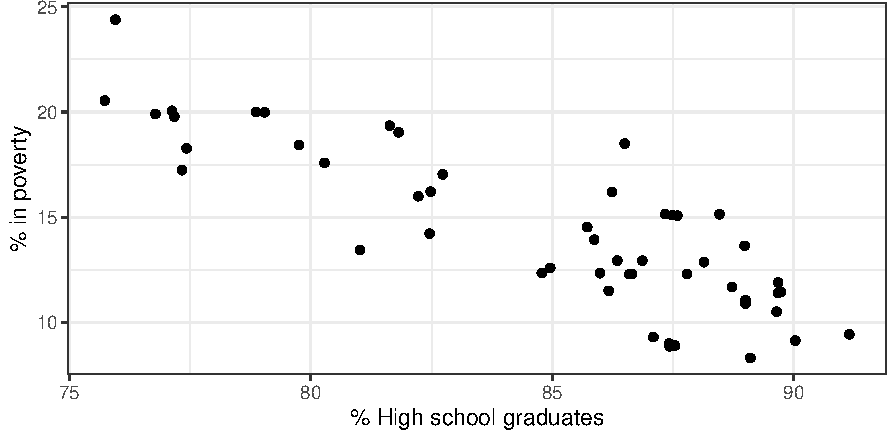
\includegraphics{forchapter5_files/figure-latex/05-poverty-1.pdf}

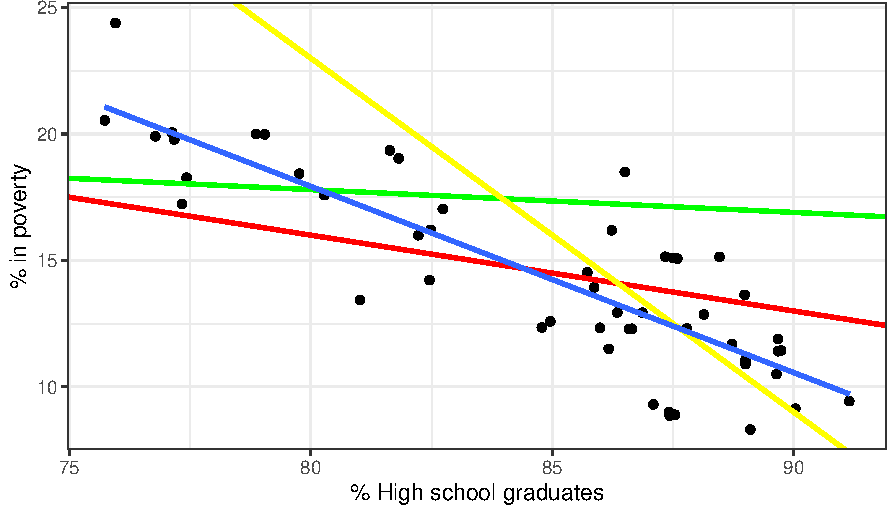
\includegraphics{forchapter5_files/figure-latex/05-eyeball-1.pdf}

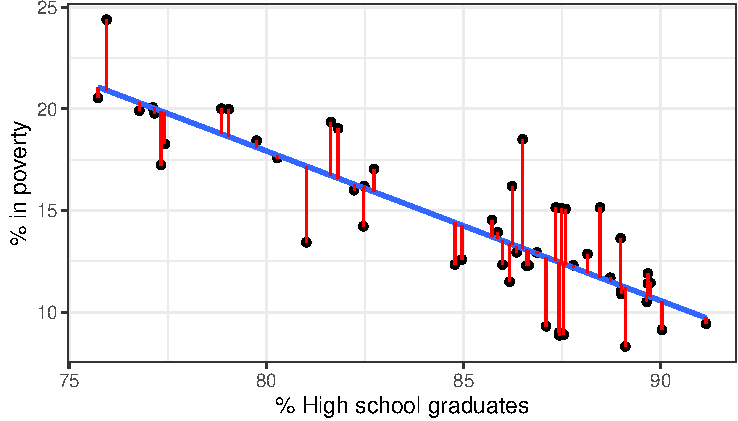
\includegraphics{forchapter5_files/figure-latex/05-minerror-1.pdf}

\end{document}
